\begin{frame}
  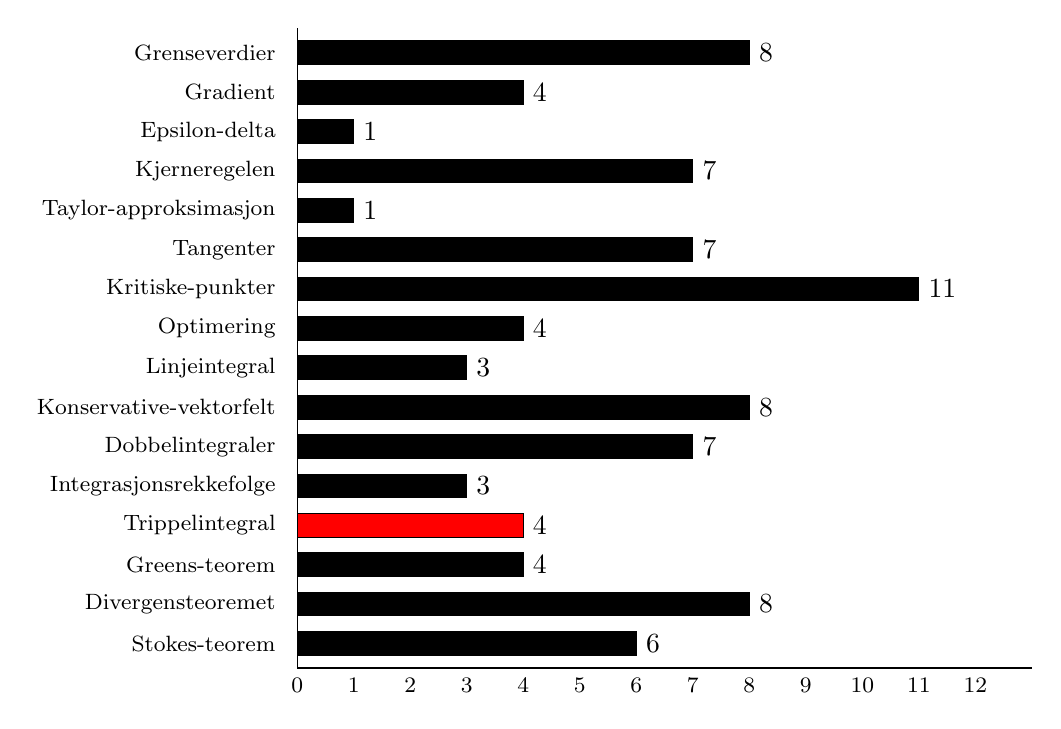
\begin{tikzpicture}
    \begin{axis}[ xbar=0pt, /pgf/bar shift=0pt, legend style={ legend columns=4,
        at={(xticklabel cs:0.5)}, anchor=north, draw=none }, ytick={0,...,15},
      ytick style={draw=none},% <- added
      axis y line*=none, axis x line*=bottom, tick label
      style={font=\footnotesize}, legend style={font=\footnotesize}, label
      style={font=\footnotesize}, xtick style={draw=none},% <- added
      xtick={0,1,...,12}, width=.9\textwidth, bar width=3mm, y dir = reverse,
      xmin=0, xmax=13, area legend,
      y=5mm, enlarge y limits={abs=0.625},
      style={text=black}, every axis plot/.append style={fill},
      nodes near coords, nodes near coords,
      yticklabels={%
        {\topicref{Grenseverdier}},
        {\topicref{Gradient}},
        {\topicref{Epsilon-delta}},
        {\topicref{Kjerneregelen}},
        {\topicref{Taylor-approksimasjon}},
        {\topicref{Tangenter}},
        {\topicref{Kritiske-punkter}},
        {\topicref{Optimering}},
        {\topicref{Linjeintegral}},
        {\topicref{Konservative-vektorfelt}},
        {\topicref{Dobbelintegraler}},
        {\topicref{Integrasjonsrekkefolge}},
        {\topicref{Trippelintegral}},
        {\topicref{Greens-teorem}},
        {\topicref{Divergensteoremet}},
        {\topicref{Stokes-teorem}}}]
      \addplot[fill=black] coordinates {(8,0)};
      \addplot[fill=black] coordinates {(4,1)};
      \addplot[fill=black] coordinates {(1,2)};
      \addplot[fill=black] coordinates {(7,3)};
      \addplot[fill=black] coordinates {(1,4)};
      \addplot[fill=black] coordinates {(7,5)};
      \addplot[fill=black] coordinates {(11,6)};
      \addplot[fill=black] coordinates {(4,7)};
      \addplot[fill=black] coordinates {(3,8)};
      \addplot[fill=black] coordinates {(8,9)};
      \addplot[fill=black] coordinates {(7,10)};
      \addplot[fill=black] coordinates {(3,11)};
      \addplot[fill=red] coordinates {(4,12)};
      \addplot[fill=black] coordinates {(4,13)};
      \addplot[fill=black] coordinates {(8,14)};
      \addplot[fill=black] coordinates {(6,15)};
    \end{axis}
  \end{tikzpicture}
\end{frame}

\begin{frame}
  \subsection{Trippelintegral}\label{subsec:Trippelintegral}
  \frametitle{Trippelintegral}
  \begin{enumerate}
    \item Tegn integrasjonsområdet i $xy$, $xz$ og $yz$-planet
    \item Bestem grensene
    \item Gjør forenklinger med hensyn på symmetri
    \item Beregn trippelintegralet og bytt grenser om nødvendig
  \end{enumerate}
\end{frame}

\begin{frame}
    \begin{oppgave}{}
    Bestem volumet til $R = \{ (x,y,z)\in\R^3 \mid 0 \leq z \leq 1 - \abs{x} - \abs{y}\}$ når
    massetettheten er gitt som $f(x,y,z) = xy + z^2$.
  \end{oppgave}
\end{frame}

\begin{frame}\centerline{Viser området avgrenset av $0 \leq z \leq 1 - \abs{x} - \abs{y}$ for
  ulike plan.}
  \centerline{%
  \includegraphics[width = 0.45\textwidth]{../img/pyramid1}%
  \includegraphics[width = 0.45\textwidth]{../img/pyramid2}}

\centerline
\visible<2>{\includegraphics[width = 0.45\textwidth]{../img/pyramid}}}
\end{frame}

\begin{frame}
    \begin{oppgave}{}
    Bestem volumet til $R = \{ (x,y,z)\in\R^3 \mid 0 \leq z \leq 1 - \abs{x} - \abs{y}\}$ når
    massetettheten er gitt som $f(x,y,z) = xy + z^n$, $n \in \mathbb{Z}$.
  \end{oppgave}
  Siden $\int_{-a}^a f(x) \dx = 0$ når $f$ er en odde funksjon, og $x$ er odde så
er $\iiint_{R}xy \dV = 0$. Da området vi integrerer over er symmetrisk. Volumet
til den blå og røde trekanten er like store, men med motsatt fortegn.
\begin{align*}
  M & = \iiint_R f(x,y,z) \dV = \iiint_R z^n \dV\\
    \only<2>{& = \int_{x=?}^{x=?} \int_{y=f(x)}^{y=g(x)}\int_{z=u(x,y)}^{z=v(x,y)} z^n \dz \dy \dx \\}
    \only<3->{& = \int_{x=-1}^{x=1} \int_{y=-1+\abs{x}}^{y=1-\abs{x}}\int_{z=0}^{z=1-\abs{x}-\abs{y}} z^n \dz \dy \dx\\}
    \visible<4->{& = 4\int_{0}^{1} \int_{0}^{1-x}\int_{0}^{1-x-y} z^n \dz \dy \dx \\}
    \visible<5->{& = 4\int_{0}^{1} \int_{0}^{1-x} \frac{(1-x-y)^{n+1}}{n+1} \dy \dx \\
    & = 4\int_{0}^{1} \frac{(1-x)^{n+2}}{(n+1)(n+2)}  \dx
      = \frac{4}{(n+1)(n+2)(n+3)}}
\end{align*}
\end{frame}




%%% Local Variables:
%%% mode: latex
%%% TeX-master: "main"
%%% End:
